\chapter{Intro}
%% Augmented reality has become a very popular topic in the last five years. With
%% the introduction of mobile smartphones, developers started to have the chance
%% to build AR applications on these devices. Between all the computer vision
%% technologies available, OpenCV and Vuforia ---specifically built for mobile
%% devices--- are among the most used. In this thesis a comparison of this technologies
%% is made with the purpose of building a mobile application to enable users to see
%% virtual posters on their walls.

Bringing augmented reality to mobile devices can be done in several ways. Getting
data from the device's camera and process its output to track a selected object is
one of the ways for querying the environment to introduce virtual elements in it. To
accomplish this, many computer vision algorithms exist and they are called object
recognition techniques.  

Using an object recognition algorithm between two images can help us to
determine whether the object we are searching for is present in the image or
not. This technique can be seen in the figure~\ref{fig:introdetect}. But, what happens if
we want to know if the object is present on a dynamic scene such as a
live video feed? We can apply the same algorithms for each of the video frame
that comes from the camera. 
Also, we can combine these object detection algorithms with the data provided
by the sensors of mobile smartphones, such as accelerometers or
gyroscopes. This data can help the algorithms to compute the user movement and
improve the tracking.

\begin{figure}
\centering
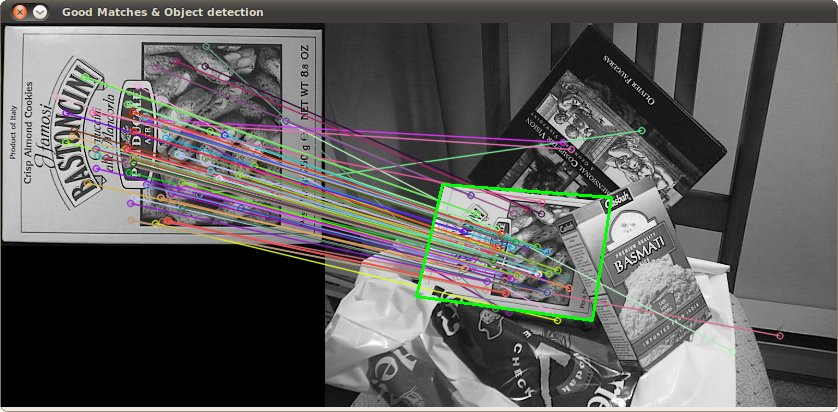
\includegraphics[scale=0.45]{img/intro-feature.jpg}
\caption{\label{fig:introdetect} Object detection using OpenCV's SURF. Taken
  from~\cite{opencvhomography}.} 
\end{figure} 

In order to determine which is the better technique to detect features in a
video feed, we present
an study of three different approximations using OpenCV algorithms and another one
using Vuforia SDK by Qualcomm\textregistered. A comparison of performance and
robustness between this four different approaches is made to decide which is the
best to bring augmented reality to a mobile environment. This comparison runs
on a real device in order to determine how this techniques behave on a limited
performance device such as a mobile smartphone.

The goal of the study is to build an augmented reality application that enables 
users to try posters on their walls using augmented reality technology. The
name given to this application is Ponster.

\section*{Structure of the work}
\subsection*{State of the art}
In this chapter we are going to explain all the techniques used in Ponster to
detect and track the object, what's the theory behind those algorithms and why
we have chosen one above another. All the OpenCV approximations are detailed:
template matching and the three feature tracking algorithms tested. Also, the
theory behind Vuforia SDK is explained.

\subsection*{Technologies}
All the technologies used to develop the Ponster app are explained in this
chapter. Both iOS-only SDKs and computer vision technologies are detailed,
from the user interface SDK to the persistency layer. Also, an extended
overview of how Vuforia works is presented.

\subsection*{Development}
In this chapter the architecture of the Ponster application is presented, along
with the model view controller hierarchy and the persistency layer. Also, a
performance comparison of all the augmented reality algorithms used is
shown. Finally, we present a detailed explaination of the Ponster features.

\subsection*{Commercial applications and future work}
We list different augmented reality applications built for mobile smartphones that
have been an inspiration to build Ponster, and we give details about how the
application can be improved with future work.

\subsection*{Conclusions}
The final part of this work is presented as a summary of all the important
things learned when bringing augmented reality ---using object tracking--- to a
power constrained device as the mobile smartphones are.
